\documentclass{beamer}

\hypersetup{pdfpagemode=FullScreen} % full screen mode
\setbeamertemplate{navigation symbols}{}

\usepackage[english]{babel}
\usepackage[latin1]{inputenc}
\usepackage{amsmath,amssymb}
\usepackage[T1]{fontenc}
\usepackage{curves}
\usepackage{verbatim}
\usepackage{multimedia}
\usepackage{mathptmx}
\usepackage{graphicx}
\usepackage{booktabs}
\usepackage{hyperref}
\usepackage{multirow}
\usepackage{xcolor}
\usepackage{algorithm,algorithmic}
\usepackage{listings}
\usepackage[font=scriptsize]{caption}
\renewcommand{\algorithmicrequire}{\textbf{Input:}}
\renewcommand{\algorithmicensure}{\textbf{Output:}}
\usepackage{lipsum}
\setbeamertemplate{caption}[numbered] % for numbering figures

\mode<presentation> {

\usetheme{Singapore}

\usecolortheme{whale}

% \setbeamertemplate{footline} % to remove the footer line in all slides uncomment this line

\setbeamertemplate{navigation symbols}{} % to remove the navigation symbols from the bottom of all slides uncomment this line
}

\usepackage{graphicx}
\usepackage{booktabs}
\setbeamercovered{transparent}
\setbeamertemplate{bibliography item}[text]
\setbeamertemplate{theorems}[numbered]
\setbeamerfont{title}{size=\Large}
\setbeamerfont{date}{size=\tiny}

\setbeamertemplate{itemize items}[ball] % if you want a ball
\setbeamertemplate{itemize subitem}[circle] % if you want a circle
\setbeamertemplate{itemize subsubitem}[triangle] % if you want a triangle

%-------Customized Frame-------
\newcounter{cont}

\makeatletter
\setbeamertemplate{frametitle continuation}{
}
\makeatother

%--------------------------
%	TITLE PAGE
%--------------------------

\title[Project I]{Project I} % the short title appears at the bottom of every slide, the full title is only on the title page

\author[Tang Quoc Thai]{\texorpdfstring{{\normalsize Tang Quoc Thai}}{Author}}

\institute[2270376] % matricola
{

{\small Supervisor: Assoc.\ Prof.\ Quan Thanh Tho}\\
\medskip
{\small Bahnaric Phoneme Segmentation}\\
%\begin{center}
%\includegraphics[width=0.1\textwidth]{uoh.png}
%\end{center}
\vspace{2cm}
\medskip
Ho Chi Minh City\\
University of Technology % your institution for the title page

%\medskip
%\textit{john@smith.com} % your email address
}
\titlegraphic{
  \begin{picture}(0,0)
    \put(22,120){\makebox(0,0)[rt]{
\includegraphics[width=1.5cm]{img/uni_logo.png}}}
  \end{picture}
  }
\date{07 Dec 2023} % date

\begin{document}
\definecolor{your_color}{HTML}{0c88dd}
\setbeamercolor{structure}{fg=your_color}

\begin{frame}
\titlepage% print the title page as the first slide
\end{frame}

\setbeamertemplate{footline}{
    \raisebox{1.5ex}[0pt][0pt]{\makebox[\paperwidth][r]{\tiny\insertpagenumber\hspace*{2ex}}}
}

%-------------------------------
%	PRESENTATION SLIDES
%-------------------------------

\section{Introduction}
\begin{frame}[allowframebreaks]
\frametitle{Motivation}
  \begin{itemize}
    \item \textbf{Objective}: Empower Bahnaric language speakers, fostering communication within their ethnic community and with other ethnic groups.
    \item \textbf{Significance of Phoneme Segmentation}:
    \begin{itemize}
      \item Create a precise phoneme-level mapping for the Bahnaric language.
      \item Enable the development of advanced Text-to-Speech (TTS) and Automatic Speech Recognition (ASR) models.
    \end{itemize}
    \item \textbf{Overall Goal}: Contribute to the empowerment and connectivity of Bahnaric ethnic communities through targeted advancements in speech processing.
  \end{itemize}
\end{frame}

\begin{frame}[allowframebreaks]
\frametitle{Bahnaric phoneme}
  \begin{columns}[T] % align columns
    \begin{column}{.5\textwidth}
      \begin{itemize}
        \item The phoneme sample consists of single words, and each word is pronounced by a native speaker.
        \item The beginning and ending time of each phoneme marked by the `ov' and `op' label respectively.
      \end{itemize}
    \end{column}%
    \begin{column}{.5\textwidth}
      \begin{block}{}
      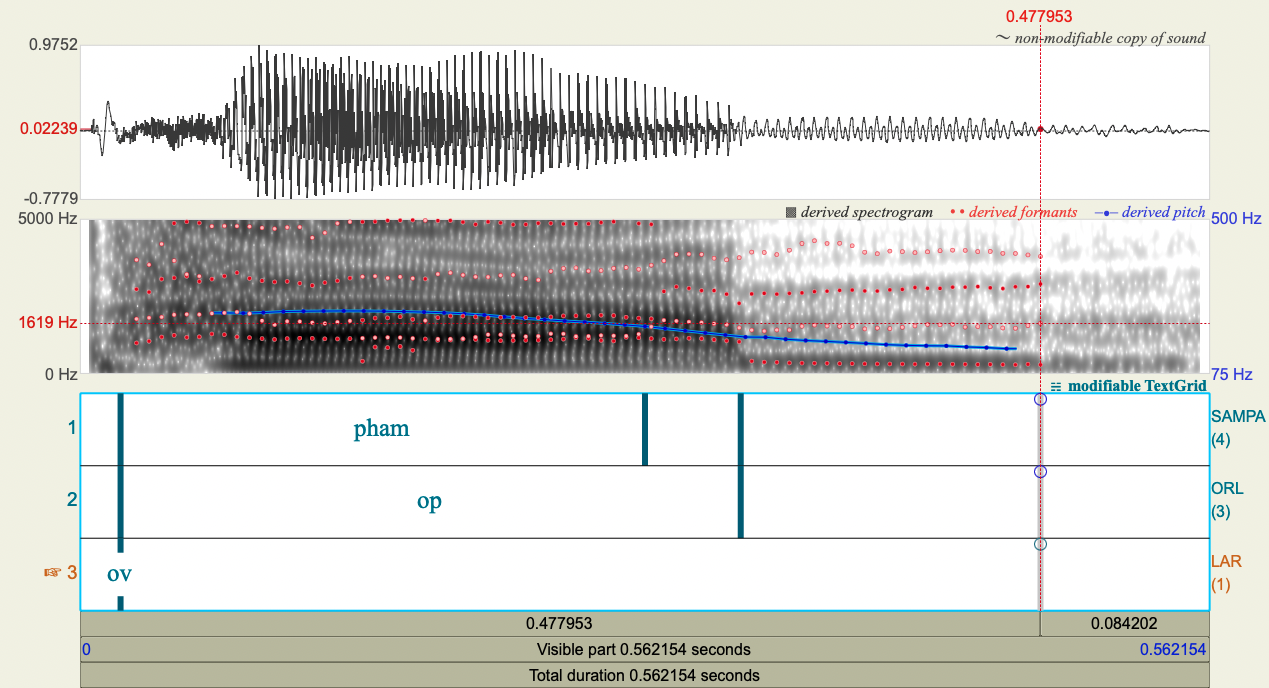
\includegraphics[width=\textwidth,height=\textheight,keepaspectratio]{img/phoneme_example.png}
      \end{block}
    \end{column}%
  \end{columns}
\end{frame}

%-------------------------------
\section{Methodology}
\begin{frame}[allowframebreaks]
\frametitle{Feature engineering}
The following features are extracted from the audio clips:
  \begin{itemize}
    \item \textbf{MFCC} (Mel Frequency Cepstral Coefficients): These are coefficients that collectively make up an MFC.\@ They are derived from a type of cepstral representation of the audio clip (a nonlinear `spectrum-of-a-spectrum').
    \item \textbf{Zero Crossings}: This is the rate at which the signal changes from positive to negative or back.
    \item \textbf{Mel Spectrogram}: A Mel Spectrogram is a spectrogram where the frequencies are converted to the Mel scale.
    \item \textbf{Harmonics}: These are integer multiples of the base frequency in a sound. They contribute to the perceived timbre of a sound.
    \item \textbf{Spectral Centroids}: It indicates where the `center of mass' of the spectrum is located. It is used in digital signal processing to identify the brightness of a sound.
    \item \textbf{Chromagram}: A chromagram is a graphical representation of the chroma of a signal. In music, the chroma of a note is its position within the octave of the twelve-note chromatic scale.
    \item \textbf{Tempo BPM} (Beats Per Minute): This is a measure of tempo in music, indicating the number of beats occurring in one minute.
    \item \textbf{Spectral Bandwidth}: This is the difference between the highest and lowest frequencies in a continuous band of frequencies. It can be used to identify the smoothness of a sound.
  \end{itemize}
\end{frame}

\begin{frame}[allowframebreaks,fragile]
\frametitle{Pseudocode of Feature engineering}
  \begin{verbatim}
for audio_clip in audio_clips:
  audio_clip_features = []
  for frame in audio_clip:
    frame_features = []
    for feature in acoustic_features:
      for window_length in range(85, 126, 10):
        windowed_audio = get_window(frame, window_length)
        mean_value = calculate_mean(window, feature)
        frame_features.append(
          {"feature_name_window_length": mean_value})
  audio_clip_features.append(
    {"audio_clip_name": frame_features})
  \end{verbatim}
\end{frame}

\begin{frame}[allowframebreaks]
\frametitle{Pseudocode of Feature engineering}
  \begin{figure}
    \centering
    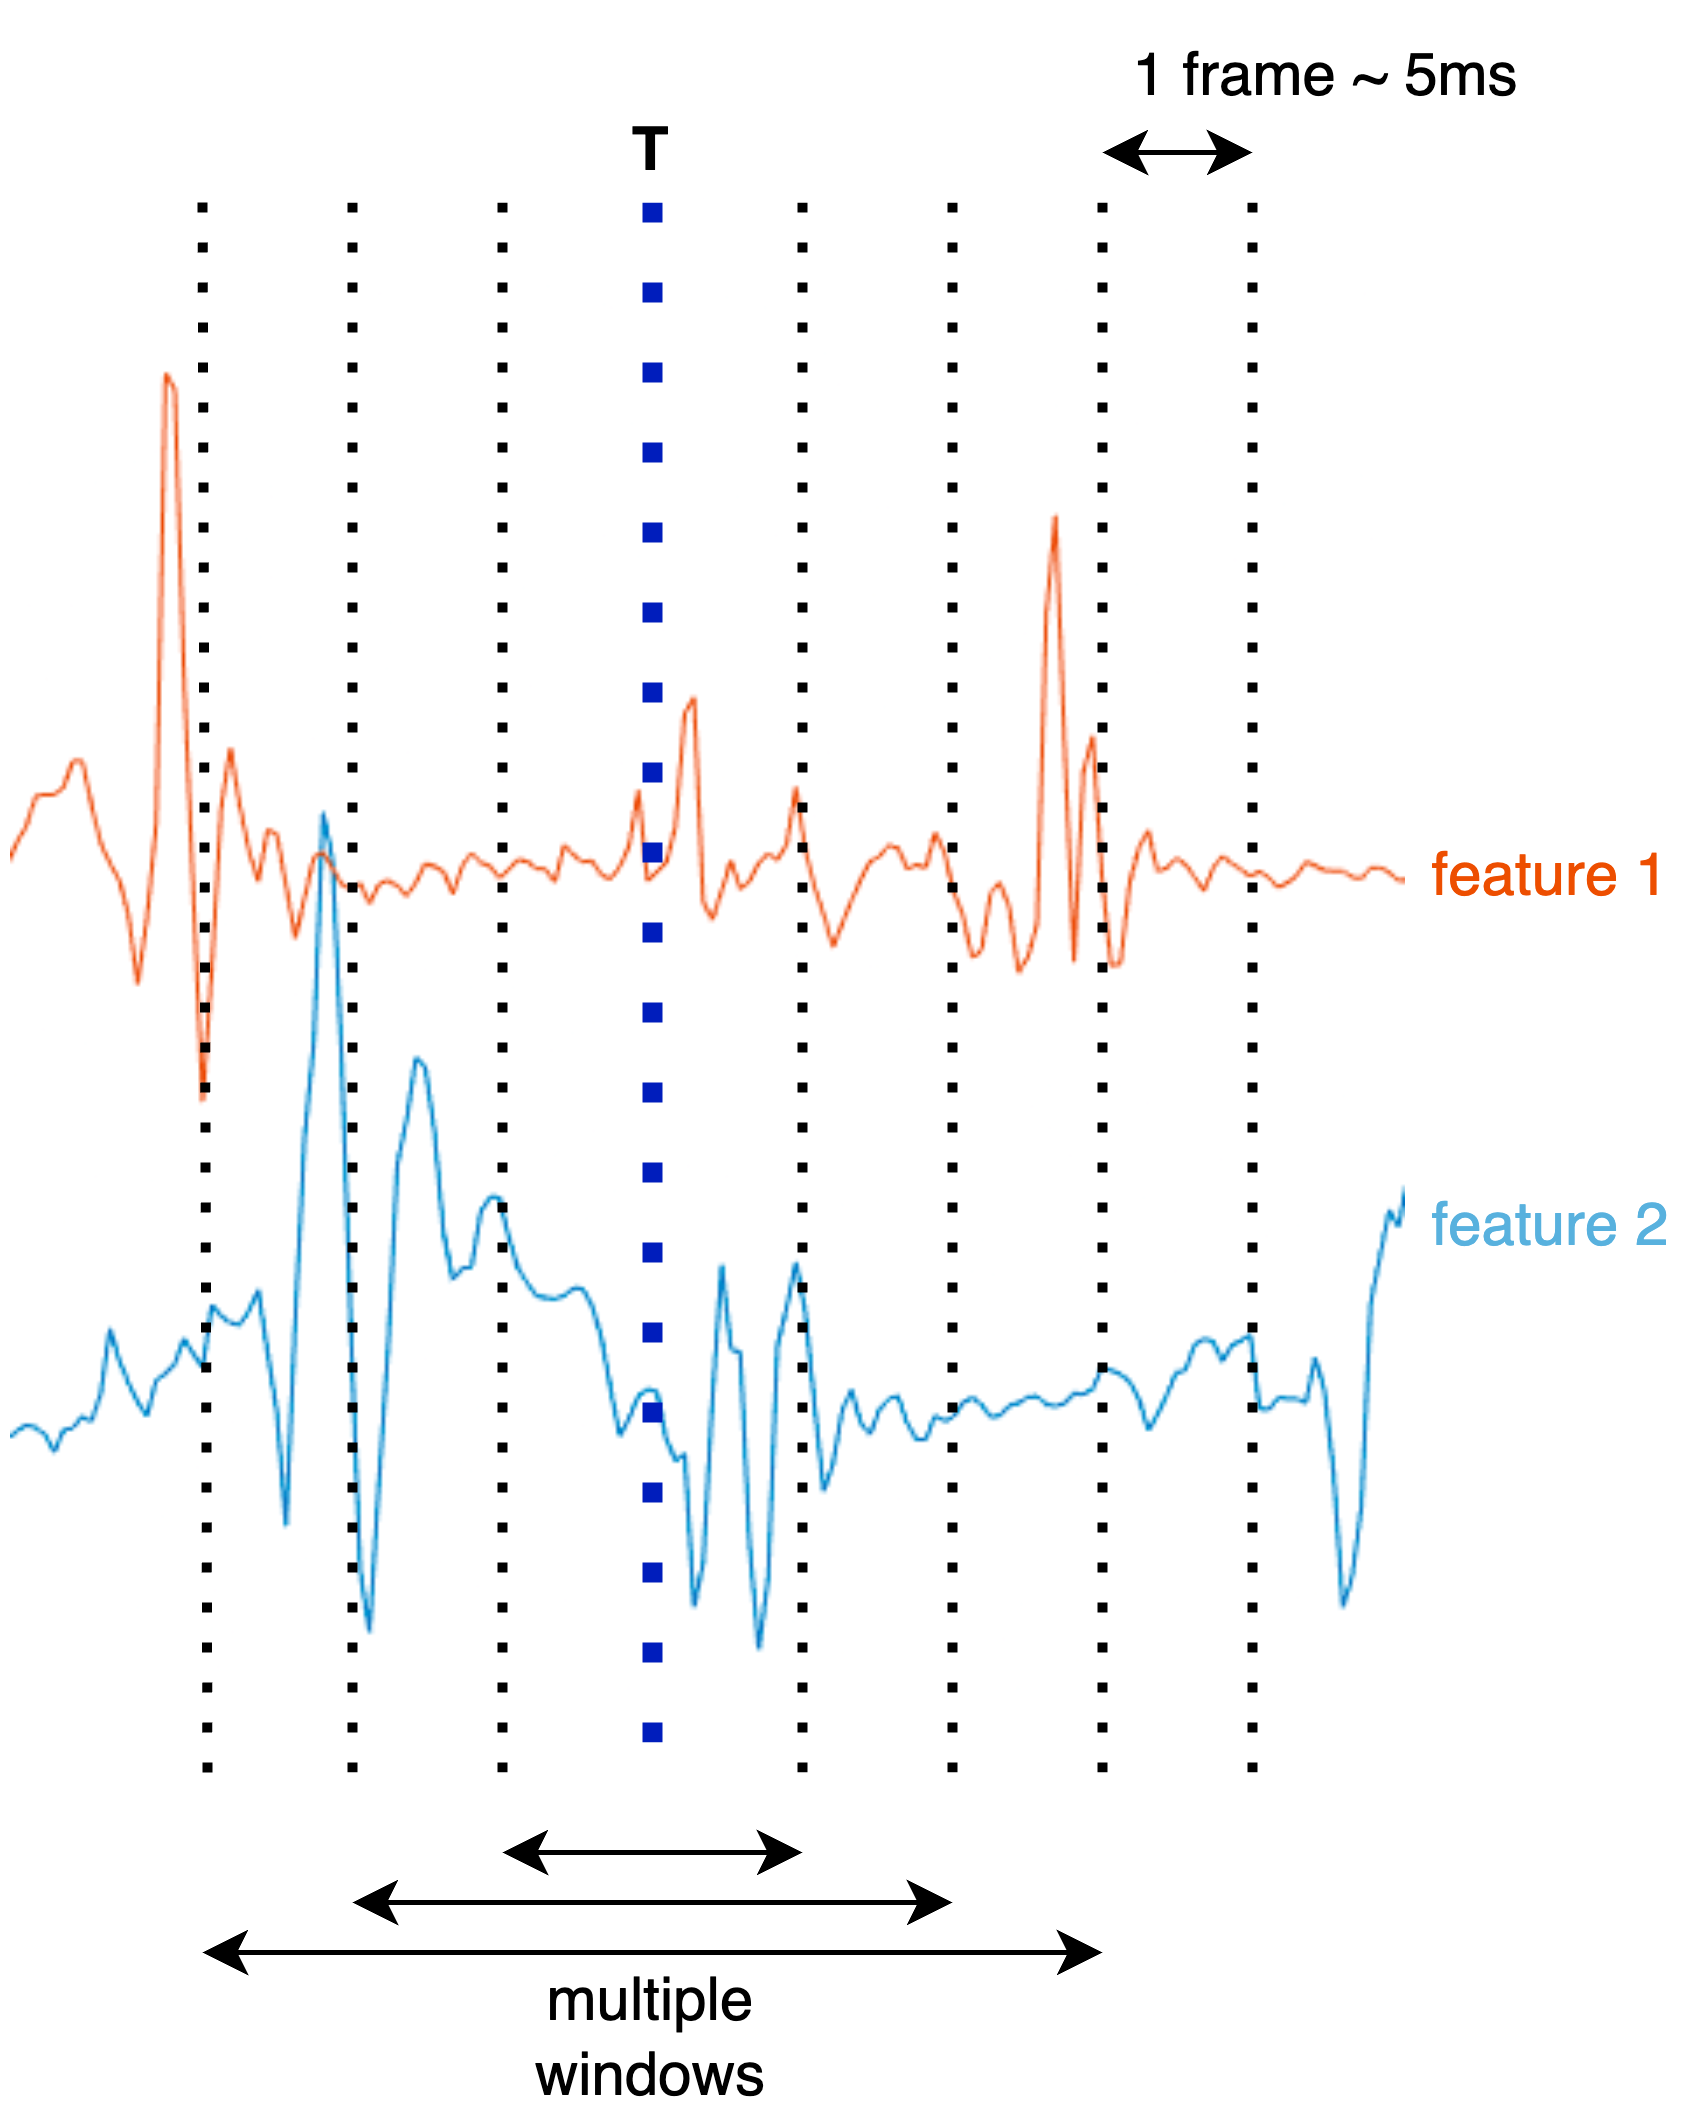
\includegraphics[width=0.5\textwidth]{img/features.png}
  \end{figure}
\end{frame}

\begin{frame}[allowframebreaks]
\frametitle{Labels}
  \begin{itemize}
    \item The `ov' and `op' labels are extracted from the TextGrid files.
    \item The information obtained reveals the timestamps of these markers in milliseconds. Consequently, it is necessary to convert these timestamps into frame indices, with each frame corresponding to a 5ms interval.
    \item \textbf{A strong assumption} has been made: the neighboring frames of the `ov' and `op' labels are also labeled as `ov' and `op' respectively.
  \end{itemize}
\end{frame}

\begin{frame}[allowframebreaks]
\frametitle{Training}
  \begin{columns}[T] % align columns
    \begin{column}{.5\textwidth}
      \begin{itemize}
        \item Each frame is treated as a data point, and the label is either 0 or 1.
        \item The extended labels are the the neighboring frames of the `ov' or `op' labels.
        \item LGBMClassifier is used to train two separate models for the `ov' and `op' labels.
      \end{itemize}
    \end{column}%
    \begin{column}{.5\textwidth}
      \begin{block}{}
      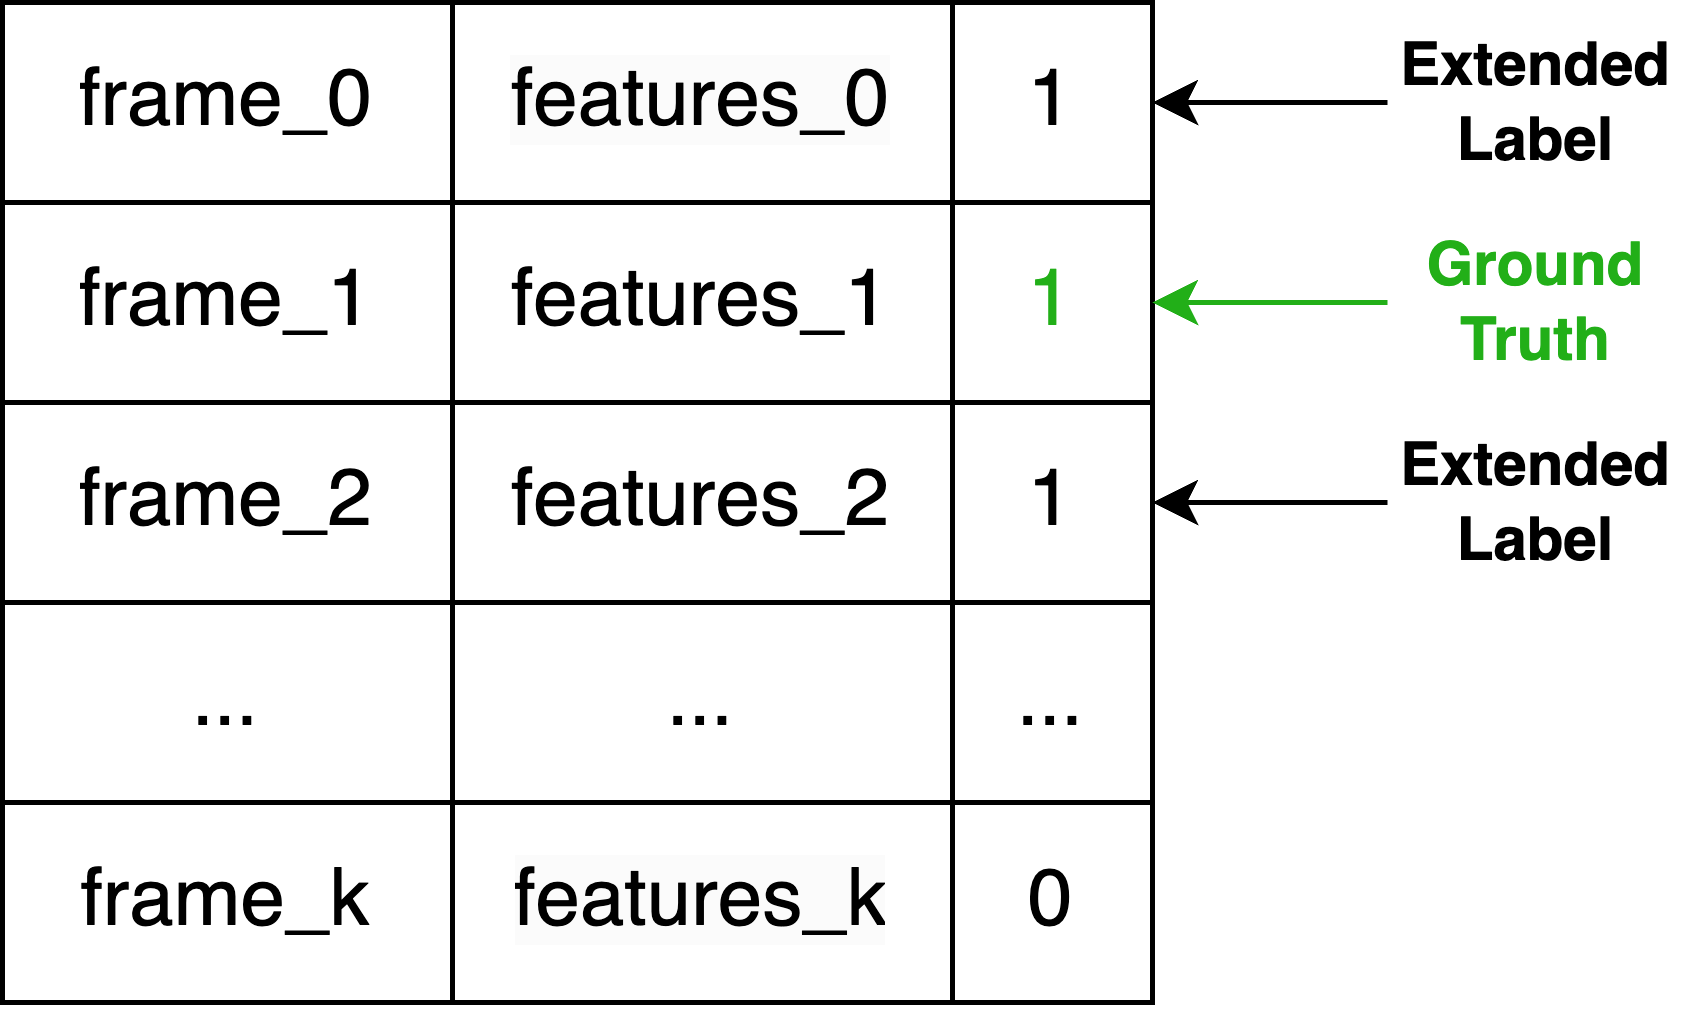
\includegraphics[width=\textwidth,height=\textheight,keepaspectratio]{img/training.png}
      \end{block}
    \end{column}%
  \end{columns}
\end{frame}

\begin{frame}[allowframebreaks]
\frametitle{Prediction}
  \begin{columns}[T] % align columns
    \begin{column}{.5\textwidth}
      \begin{itemize}
        \item The trained model is used to predict the probability of each frame being labeled as `ov' or `op'.
        \item The only frame with the highest probability and larger than 0.5 is selected as the `ov' or `op' label.
      \end{itemize}
    \end{column}%
    \begin{column}{.5\textwidth}
      \begin{block}{}
      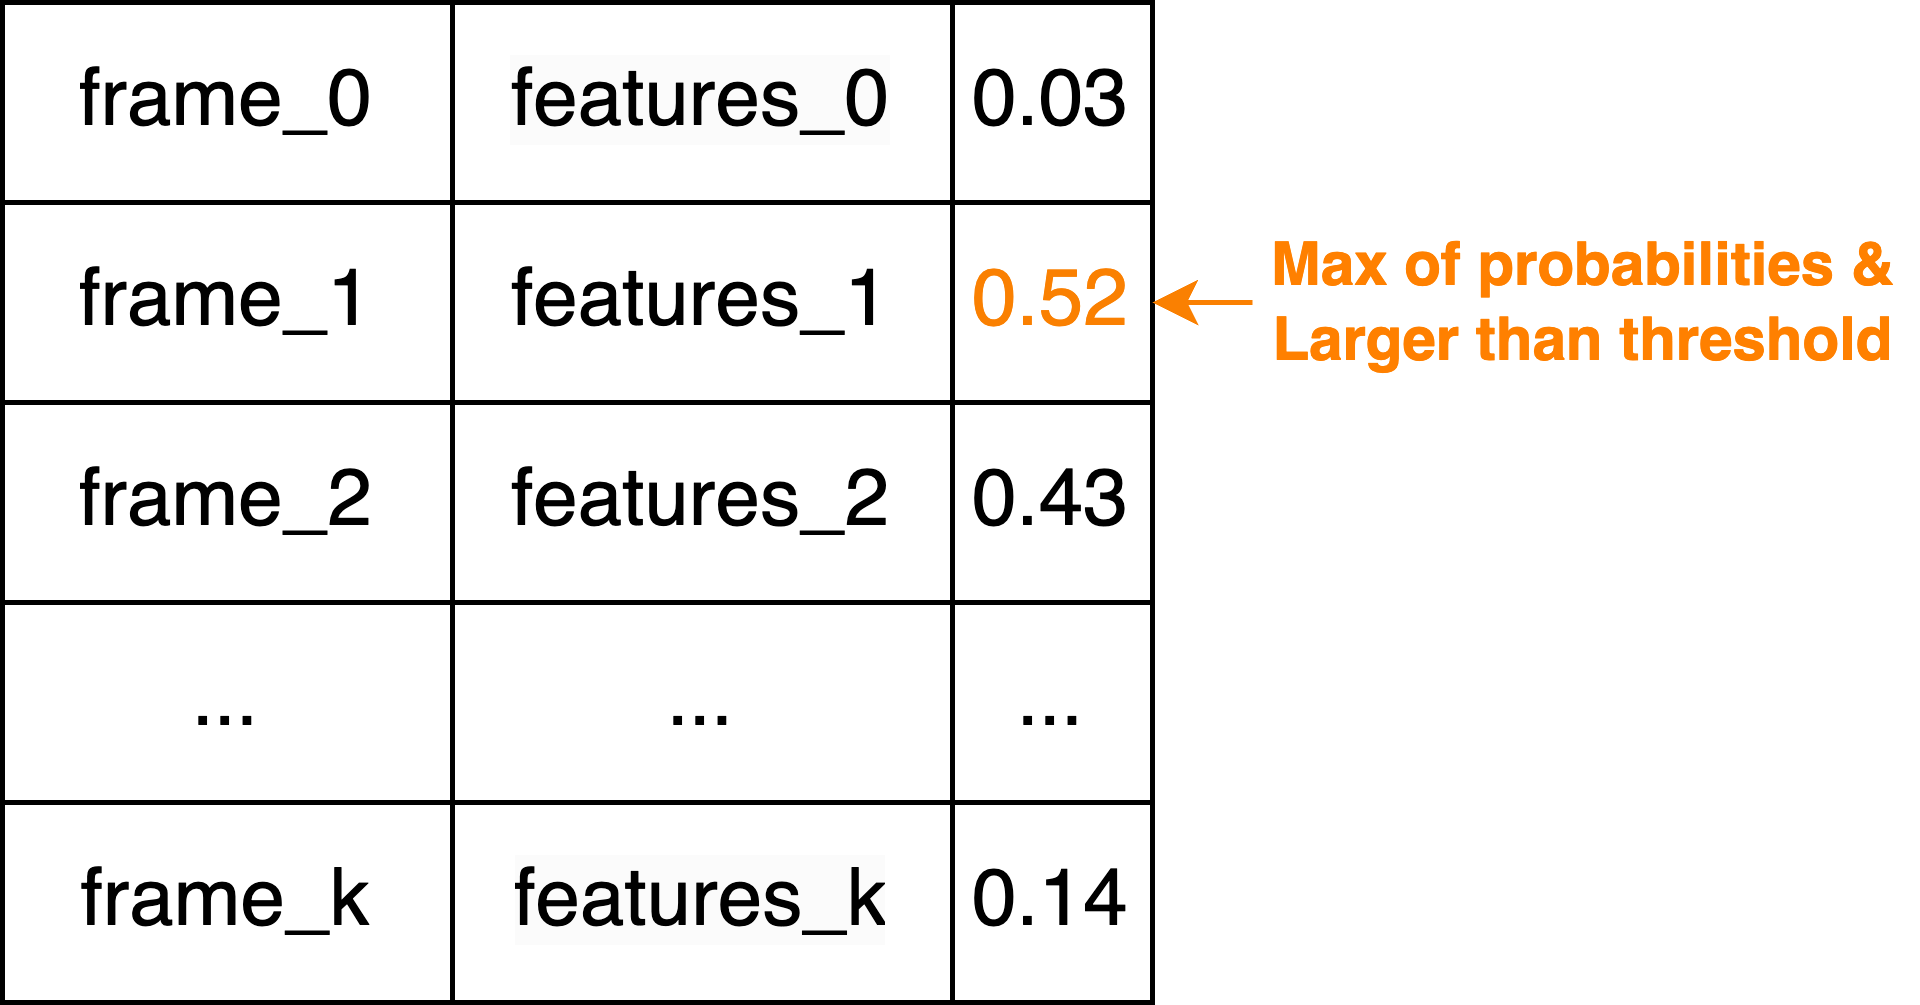
\includegraphics[width=\textwidth,height=\textheight,keepaspectratio]{img/prediction.png}
      \end{block}
    \end{column}%
  \end{columns}
\end{frame}

%-------------------------------
\section{Result}
\begin{frame}[allowframebreaks]
\frametitle{Result}\scriptsize
  \begin{itemize}
    \item The model is trained on 80\% of the data and tested on the remaininng 20\%.
    \item The model achieves an accuracy of 0.67 and 0.79 for the `ov' and `op' labels respectively.
  \end{itemize}

  \begin{table}[h]
    \centering
    \begin{tabular}{l c c c}
    \midrule
    & Precision & Recall & Accuracy \\
    op & 0.78 & 0.38 & 0.67 \\
    ov & 0.76 & 0.60 & 0.79 \\
    \midrule
    \end{tabular}
  \end{table}
\end{frame}

%-------------------------------
\begin{frame}
\Huge{\centerline{Thank You}}
\end{frame}
\end{document}
